\documentclass{article}
\usepackage{graphicx}
\usepackage{amsmath}
\usepackage{amssymb}
\usepackage{mathtools}
\usepackage{datetime}
\usepackage{lipsum}
\graphicspath{{images/}}

\setlength\parindent{0pt}	% no indent for entire document

\title{Backpropagation for FC Neural Network}

\newcommand\blfootnote[1]
{%
  \begingroup
  \renewcommand\thefootnote{}\footnote{#1}%
  \addtocounter{footnote}{-1}%
  \endgroup
}
 
\begin{document}

\begin{titlepage}
\author{Hao Huang}
\date{\today}
\maketitle
\end{titlepage}

\tableofcontents
\newpage

\section{Network Structure}
\begin{center}
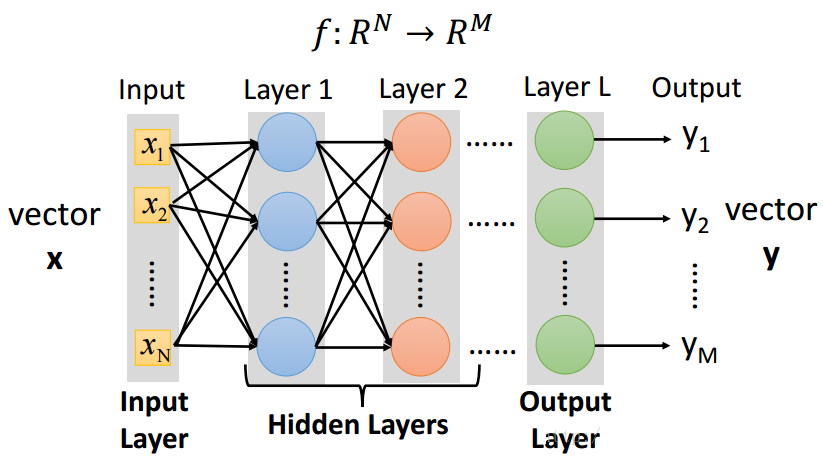
\includegraphics[scale=0.3]{neuralnetwork}
\end{center} 

\blfootnote{Credit and Copyright:}
\blfootnote{http://blog.csdn.net/sysstc/article/details/75305276}
\blfootnote{http://blog.csdn.net/sysstc/article/details/75269563}
 
\section{Notations}
\subsection{Output of activation}
\begin{center}
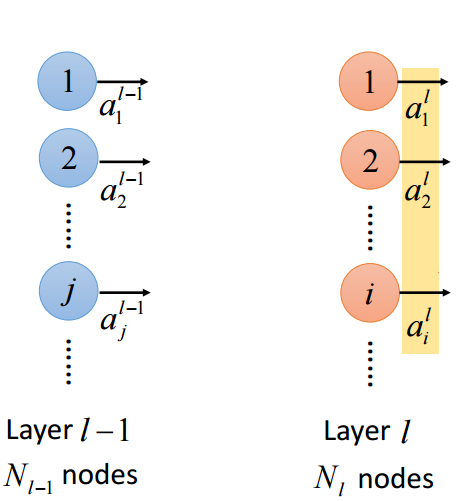
\includegraphics[scale=0.3]{activation_output}
\end{center}
Output of a neuron: $a^l_i$ (Superscript $l$ is the layer, and subscript is the index in layer)

Output of a layer: $a^l$ (a vector)

\subsection{Weights}
\begin{center}
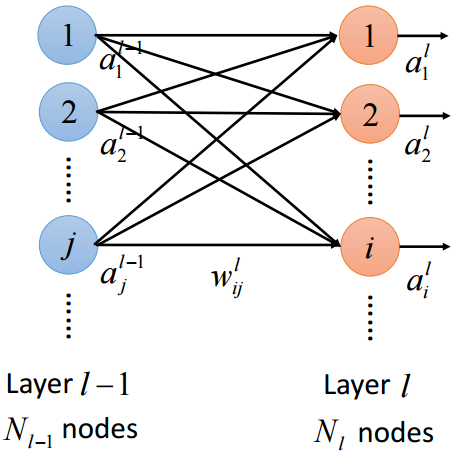
\includegraphics[scale=0.4]{weights}
\end{center}
$w^l_{ij}$: from neuron $j$ (layer $l-1$) to neuron $i$ (layer $l$)

\[
W^l
=
\begin{bmatrix}
    w^l_{11} & w^l_{12} & \dots & w^l_{1j} & \dots  & w^l_{1N_{l-1}} \\
    w^l_{21} & w^l_{22} & \dots & w^l_{2j} & \dots  & w^l_{2N_{l-1}} \\
    \vdots & \vdots & \vdots & \vdots & \ddots & \vdots \\
    w^l_{N_l1} & w^l_{N_l2} & \dots & w^l_{N_lj} & \dots & w^l_{N_lN_{l-1}}
\end{bmatrix}_{N_l\times N_{l-1}}
\]

\subsection{Biases}
\begin{center}
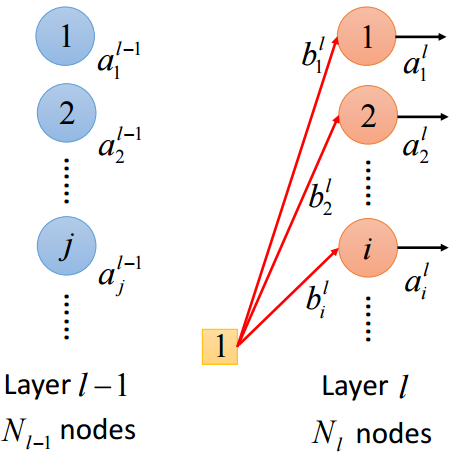
\includegraphics[scale=0.4]{biases}
\end{center}
$b^l_i$: bias for neuron $i$ at layer $l$
\[
b^l
=
\begin{bmatrix}
    b^l_{1} & b^l_{2} & \dots & b^l_{i} & \dots  & b^l_{N_l}
\end{bmatrix}^T
\]

\subsection{Input of activation}
\begin{center}
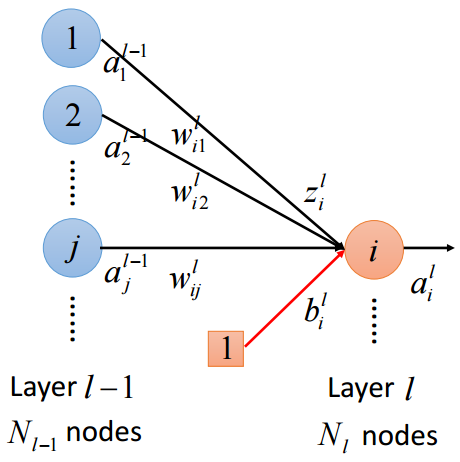
\includegraphics[scale=0.4]{activation_input}
\end{center}
$z^l_i$: input of the activation function of neuron $i$ at layer $l$

$z^l$: input of the activation function of all neurons at layer $l$

\[
z^l_i = \sum_j^{N_{l-1}} w^l_{ij}a^{l-1}_j + b^l_i
\]

\[
z^l = 
\begin{bmatrix}
    z^l_{1} & z^l_{2} & \dots & z^l_{i} & \dots  & z^l_{N_l}
\end{bmatrix}^T
\]

\subsection{Relations between layers}
\begin{center}
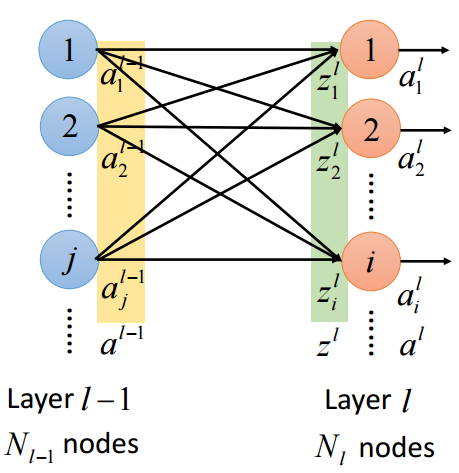
\includegraphics[scale=0.4]{layer_1}
\end{center}
\[
z^l_1 = w^l_{11}a^{l-1}_1 + w^l_{12}a^{l-1}_2 + \dots + w^l_{1j}a^{l-1}_j + \dots + w^l_{1N_{l-1}}a^{l-1}_{N_{l-1}} + b^l_1
\]
\[
z^l_2 = w^l_{21}a^{l-1}_1 + w^l_{22}a^{l-1}_2 + \dots + w^l_{2j}a^{l-1}_j + \dots + w^l_{2N_{l-1}}a^{l-1}_{N_{l-1}} + b^l_2
\]
\[
\vdots
\]
\[
z^l_i = w^l_{i1}a^{l-1}_1 + w^l_{i2}a^{l-1}_2 + \dots + w^l_{ij}a^{l-1}_j + \dots + w^l_{iN_{l-1}}a^{l-1}_{N_{l-1}} + b^l_i
\]
\[
\vdots
\]
\[
z^l_{N_l} = w^l_{N_l1}a^{l-1}_1 + w^l_{N_l2}a^{l-1}_2 + \dots + w^l_{N_lj}a^{l-1}_j + \dots + w^l_{N_lN_{l-1}}a^{l-1}_{N_{l-1}} + b^l_{N_l}
\]
Rewrite them as matrix multiplication form:
\[
\begin{bmatrix}
z^l_{1} \\ z^l_{2} \\ \vdots \\ z^l_{i} \\ \vdots  \\ z^l_{N_l}
\end{bmatrix}
=
\begin{bmatrix}
    w^l_{11} & w^l_{12} & \dots & w^l_{1j} & \dots  & w^l_{1N_{l-1}} \\
    w^l_{21} & w^l_{22} & \dots & w^l_{2j} & \dots  & w^l_{2N_{l-1}} \\
    \vdots & \vdots & \ddots & \vdots & \ddots & \vdots \\
    w^l_{i1} & w^l_{i2} & \dots & w^l_{ij} & \dots  & w^l_{iN_{l-1}} \\
    \vdots & \vdots & \ddots & \vdots & \ddots & \vdots \\
    w^l_{N_l1} & w^l_{N_l2} & \dots & w^l_{N_lj} & \dots & w^l_{N_lN_{l-1}}
\end{bmatrix}
\begin{bmatrix}
a^{l-1}_{1} \\ a^{l-1}_{2} \\ \vdots \\ a^{l-1}_{j} \\ \vdots  \\ a^{l-1}_{N_{l-1}}
\end{bmatrix}
+
\begin{bmatrix}
b^l_{1} \\ b^l_{2} \\ \vdots \\ b^l_{i} \\ \vdots  \\ b^l_{N_l}
\end{bmatrix}
\]
That is:
\[
z^l = W^l a^{l-1} + b^l
\]

\begin{center}
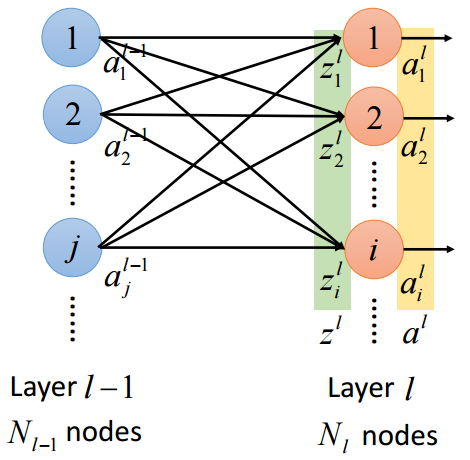
\includegraphics[scale=0.4]{layer_2}
\end{center}
For neuron $i$ in layer $l$:
\[
a^l_i = \sigma(z^l_i)
\]
For the layer $l$:
\[
\begin{bmatrix}
a^l_{1} \\ a^l_{2} \\ \vdots \\ a^l_{i} \\ \vdots  \\ a^l_{N_l}
\end{bmatrix}
=
\begin{bmatrix}
\sigma(z^l_1) \\ \sigma(z^l_2) \\ \vdots \\ \sigma(z^l_i) \\ \vdots  \\ \sigma(z^l_{N_l})
\end{bmatrix}
\]
Rewrite it as:
\[
a^l = \sigma(z^l)
\]

\begin{center}
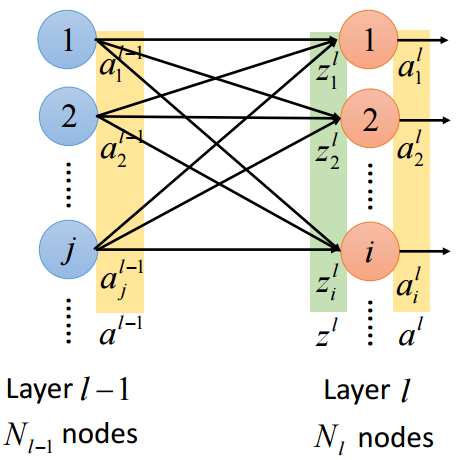
\includegraphics[scale=0.4]{layer_3}
\end{center}
\[
\begin{rcases*}
a^l = \sigma(z^l)\\
z^l = W^l a^{l-1} + b^l
\end{rcases*} \Rightarrow a^l=\sigma(W^la^{l-1}+b^l)
\]

\subsection{Summary of notation}
\begin{center}
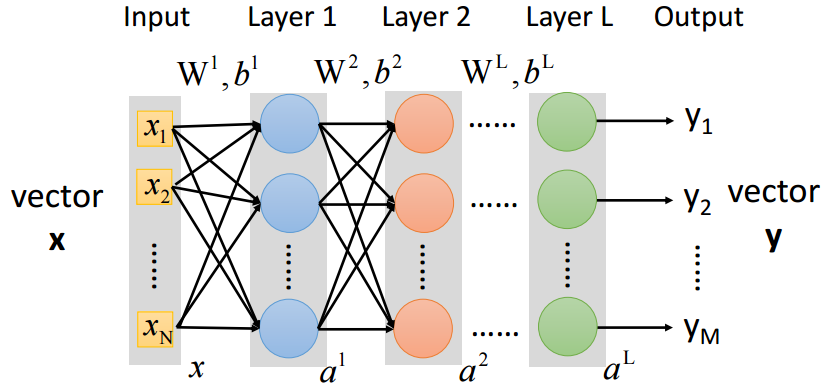
\includegraphics[scale=0.4]{notation_1}
\end{center}
\[
a^1=\sigma(W^1x+b^1)
\]
\[
a^2=\sigma(W^2a^1+b^2)
\]
\[
\vdots
\]
\[
y=a^L=\sigma(W^{L}a^{L-1}+b^L)
\]
Consider a neural network as a function:
\[
y=f(x)=\sigma(W^L...\sigma(W^2\sigma(W^1x+b^1)+b^2)...+b^L)
\]

\section{Three gradient descent approaches}
$\theta$ is the parameter set of a neural network (e.g. $\{W^1, b^1, ..., W^L, b^L\}$), and $C$ is the cost function. The superscript $i$ indicates the $i$-th update. $N$ is the number of training samples.
\subsection{Gradient descent}
\[
\theta^i = \theta^{i-1} - \eta\nabla C(\theta^{i-1})
\]
\[
\nabla C(\theta^{i-1}) = \frac{1}{N}\sum_{r = 1}^N\nabla C _r(\theta^{i-1})
\]
\subsection{Stochastic gradient descent}
Randomly pick a training sample $x_r$:
\[
\theta^i = \theta^{i-1} - \eta \nabla C_r(\theta^{i-1})
\]
\subsection{Mini-batch gradient descent}
Shuffle the training data and then pick $M$ samples as a batch:
\[
\theta^i = \theta^{i-1} - \eta \frac{1}{M}\sum_{x_r\in batch}\nabla C_r(\theta^{i-1})
\]

\section{Backpropagation}
The change in $w^l_{ij}$ leads to the change in $C_r$, so we need to compute $\nabla C_r$ with respect to $w^l_{ij}$.

\subsection{Partial derivative of $C_r$ w.r.t $w^l_{ij}$}
\begin{center}
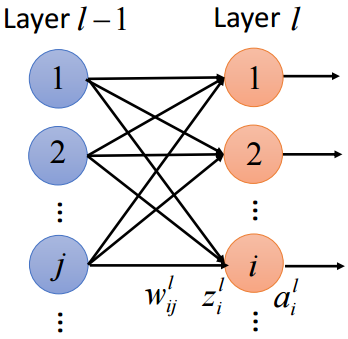
\includegraphics[scale=0.4]{grad_ctow}
\end{center}
\[
\Delta w^l_{ij}\rightarrow \Delta z^l_i\rightarrow \Delta a^l_i \rightarrow \dots \rightarrow \Delta C_r 
\]
\[
\frac{\partial C_r}{\partial w^l_{ij}} = \frac{\partial C_r}{\partial z^l_i}\frac{\partial z^l_i}{\partial w^l_{ij}}
\]

\subsection{Partial derivative of $z^l_i$ w.r.t $w^l_{ij}$}
We divide this partial derivative into two parts: input layer and hidden layer(s).

\subsubsection{Input layer}
Suppose the input layer has $N_0$ input nodes. The superscript $r$ of $x$ means the $r$-th sample.
\begin{center}
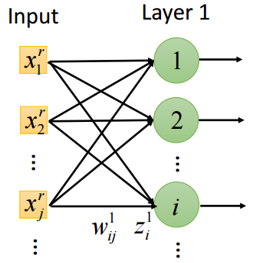
\includegraphics[scale=0.5]{grad_ztow_input}
\end{center}
\[
z^1_i = \sum_j^{N_0}w^1_{ij}x^r_j + b^1_i
\]
\[
\frac{\partial z^1_i}{\partial w^1_{ij}} = x^r_j
\]

\subsubsection{Hidden layer}
\begin{center}
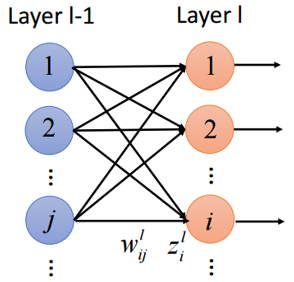
\includegraphics[scale=0.5]{grad_ztow_hidden}
\end{center}
\[
z^l_i = \sum_j^{N_{l-1}}w^l_{ij}a^{l-1}_j + b^l_i
\]
\[
\frac{\partial z^l_i}{\partial w^l_{ij}} = a^{l-1}_j
\]

\subsection{Partial derivative of $C_r$ w.r.t $z^l_{i}$}
\[
\frac{\partial C_r}{\partial w^l_{ij}} = \frac{\partial C_r}{\partial z^l_i}\frac{\partial z^l_i}{\partial w^l_{ij}}
\]
We denote $\frac{\partial C_r}{\partial z^l_i}$ as $\delta^l_i$ and define $\delta^l = [\delta^l_1 \: \delta^l_2 \: \dots \delta^l_i \: \dots \: \delta^l_{N_l}]^T$.

\begin{center}
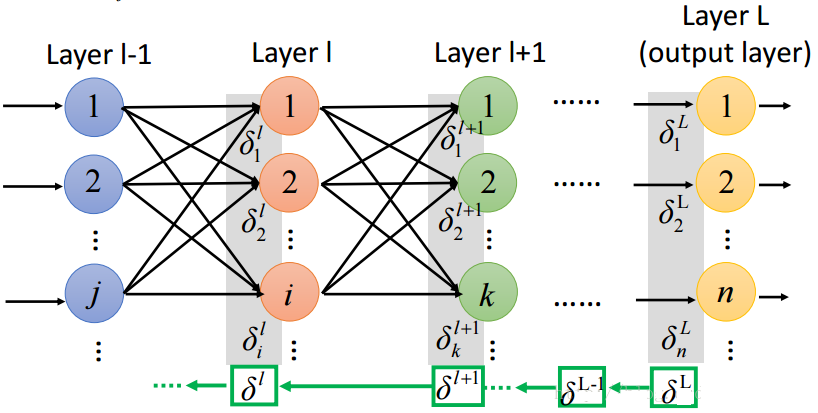
\includegraphics[scale=0.4]{delta}
\end{center}

We need to compute $\delta^l$. However, computing $\delta^l$ can be divided into two steps:
\begin{enumerate}
\item
computing $\delta^L$ (output layer)
\item
figuring out the relationship between $\delta^{l+1}$ and $\delta^l$ 
\end{enumerate}

\subsubsection{Computing $\delta^L$ (output layer)} 
\begin{center}
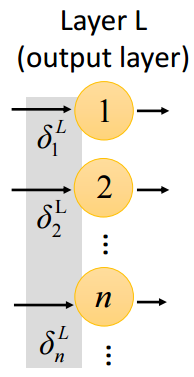
\includegraphics[scale=0.5]{grad_last}
\end{center}
\[
\Delta z^L_n\rightarrow \Delta a^L_n = \Delta y^r_n \rightarrow \Delta C_r 
\]
\[
\delta^L_n = \frac{\partial C_r}{\partial z^L_n} = \frac{\partial C_r}{\partial y^r_n}\frac{\partial y^r_n}{\partial z^L_n} = \frac{\partial C_r}{\partial y^r_n}\sigma^\prime(z^L_n)
\]
In addition, $\frac{\partial C_r}{\partial y^r_n}$ depends on the definition of the cost function.
\[
\delta^L
=
\begin{bmatrix}
\delta^L_1 \\ \delta^L_2 \\ \vdots \\ \delta^L_n \\ \vdots  \\ \delta^L_{N_L})
\end{bmatrix}
=
\begin{bmatrix}
(\partial C_r \mathbin{/} \partial y^r_1)\times\sigma^\prime(z^L_1) \\ 
(\partial C_r \mathbin{/} \partial y^r_2)\times\sigma^\prime(z^L_2) \\
\vdots \\
(\partial C_r \mathbin{/} \partial y^r_n)\times\sigma^\prime(z^L_n) \\
\vdots \\
(\partial C_r \mathbin{/} \partial y^r_{N_L})\times\sigma^\prime(z^L_{N_L})
\end{bmatrix}
=
\begin{bmatrix}
(\partial C_r \mathbin{/} \partial y^r_1) \\ 
(\partial C_r \mathbin{/} \partial y^r_2) \\
\vdots \\
(\partial C_r \mathbin{/} \partial y^r_n) \\
\vdots \\
(\partial C_r \mathbin{/} \partial y^r_{N_L})
\end{bmatrix}
\odot
\begin{bmatrix}
\sigma^\prime(z^L_1) \\ \sigma^\prime(z^L_2) \\ \vdots \\
\sigma^\prime(z^L_n) \\ \vdots \\ \sigma^\prime(z^L_{N_L})
\end{bmatrix}
\]
$\odot$ is element-wise multiplication. We rewrite this formula is a vector form:
\[
\delta^L = \nabla C_r(y^r) \odot \sigma^\prime(z^L)
\]

\subsubsection{Relationship between $\delta^{l+1}$ and $\delta^l$} 
\begin{center}
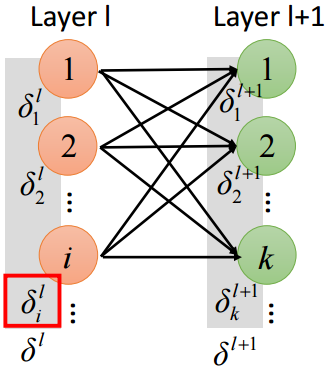
\includegraphics[scale=0.6]{grad_delta}
\end{center}
Because the output of $i$-th node in layer $l$ (e.g., $a^l_i$) will be passed in to every node in layer $l+1$, so we have:
\[
\Delta z^l_i \rightarrow \Delta a^l_i \rightarrow 
\begin{dcases*}
\begin{rcases*}
\Delta z^{l+1}_1 \\ \Delta z^{l+1}_2 \\ \vdots \\ \Delta z^{l+1}_k \\ \vdots \\ \Delta z^{l+1}_{N_{l+1}} 
\end{rcases*} 
\end{dcases*} \dashrightarrow \Delta C_r
\]
\[
\delta^l_i = \frac{\partial C_r}{\partial z^l_i} = \sum^{N_{l+1}}_k\frac{\partial C_r}{\partial z^{l+1}_k}\frac{\partial z^{l+1}_k}{\partial a^l_i}\frac{\partial a^l_i}{\partial z^l_i} = \frac{\partial a^l_i}{\partial z^l_i}\sum^{N_{l+1}}_k\frac{\partial C_r}{\partial z^{l+1}_k}\frac{\partial z^{l+1}_k}{\partial a^l_i} = \frac{\partial a^l_i}{\partial z^l_i}\sum^{N_{l+1}}_k\delta^{l+1}_k\frac{\partial z^{l+1}_k}{\partial a^l_i}
\]
\[
\because a^l_i = \sigma(z^l_i) \; \land \; z^{l+1}_k = \sum^{N_l}_i w^{l+1}_{ki}a^l_i + b^{l+1}_k
\] 
\[
\therefore \delta^l_i = \sigma^\prime(z^l_i)\sum^{N_{l+1}}_k\delta^{l+1}_kw^{l+1}_{ki} = \sigma^\prime(z^l_i)\sum^{N_{l+1}}_kw^{l+1}_{ki}\delta^{l+1}_k
\]
Let us rewrite it in vector (and matrix) form:
\[
\sigma^\prime(z^l)
=
\begin{bmatrix}
\sigma^\prime(z^l_1) \\ \sigma^\prime(z^l_2) \\ \vdots \\
\sigma^\prime(z^l_i) \\ \vdots \\ \sigma^\prime(z^l_{N_l})
\end{bmatrix}
\; \land \;
\delta^{l+1}
=
\begin{bmatrix}
\delta^{l+1}_1 \\ \delta^{l+1}_2 \\ \vdots \\
\delta^{l+1}_k \\ \vdots \\ \delta^{l+1}_{N_{l+1}}
\end{bmatrix}
\] 
\[
\delta^l
=
\begin{bmatrix}
\delta^l_1 \\ \delta^l_2 \\ \vdots \\
\delta^l_i \\ \vdots \\ \delta^l_{N_l}
\end{bmatrix}
=
\begin{bmatrix}
\sigma^\prime(z^l_1) \\ \sigma^\prime(z^l_2) \\ \vdots \\
\sigma^\prime(z^l_i) \\ \vdots \\ \sigma^\prime(z^l_{N_l})
\end{bmatrix}
\odot
\begin{pmatrix} 
\begin{bmatrix}
w^{l+1}_{11} & w^{l+1}_{21} & \dots & w^{l+1}_{k1} & \dots & w^{l+1}_{N_{l+1}1}\\
w^{l+1}_{12} & w^{l+1}_{22} & \dots & w^{l+1}_{k2} & \dots & w^{l+1}_{N_{l+1}2}\\
\vdots & \vdots & \ddots & \vdots & \ddots & \vdots\\
w^{l+1}_{1i} & w^{l+1}_{2i} & \dots & w^{l+1}_{ki} & \dots & w^{l+1}_{N_{l+1}i}\\
\vdots & \vdots & \ddots & \vdots & \ddots & \vdots\\
w^{l+1}_{1N_l} & w^{l+1}_{2N_l} & \dots & w^{l+1}_{kN_l} & \dots & w^{l+1}_{N_{l+1}N_l}\\
\end{bmatrix}
\begin{bmatrix}
\delta^{l+1}_1 \\ \delta^{l+1}_2 \\ \vdots \\
\delta^{l+1}_k \\ \vdots \\ \delta^{l+1}_{N_{l+1}}
\end{bmatrix}
\end{pmatrix}
\]
That is:
\[
\delta^l = \sigma^\prime(z^l)\odot[(W^{l+1})^T\delta^{l+1}]
\]
Thus we get the relationship between $\delta^{l+1}$ and $\delta^l$.

\subsubsection{Another viewpoint}
From this formula: $\delta^l_i = \sigma^\prime(z^l_i)\sum^{N_{l+1}}_kw^{l+1}_{ki}\delta^{l+1}_k$, we can view it as a new type of neuron, where $\sigma^\prime(z^l_i)$ is an "amplifier".
\begin{center}
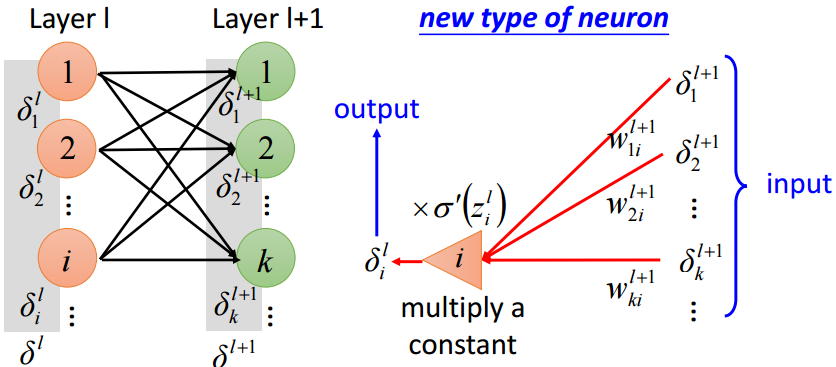
\includegraphics[scale=0.6]{new_neuron}
\end{center}
The relationship between the layer $l$ and layer $l+1$ (e.g., $\delta^l = \sigma^\prime(z^l)\odot[(W^{l+1})^T\delta^{l+1}]$) can be viewed as:
\begin{center}
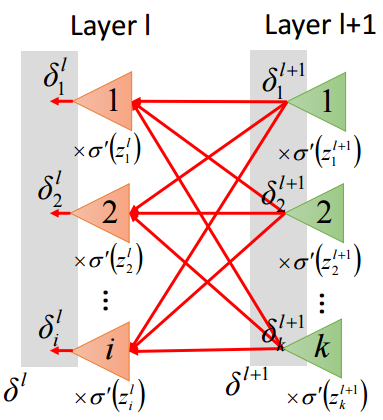
\includegraphics[scale=0.6]{new_layer}
\end{center}
Now we compare the forward-pass network and the backward-pass network:
\begin{enumerate}
\item
Forward-pass network
\begin{center}
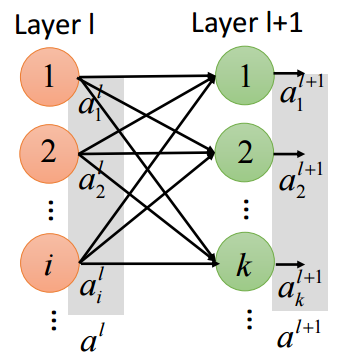
\includegraphics[scale=0.4]{forward}
\end{center}
\[
a^{l+1} = \sigma(W^{l+1}a^l+b^{l+1})
\]
\item
Backward-pass network
\begin{center}
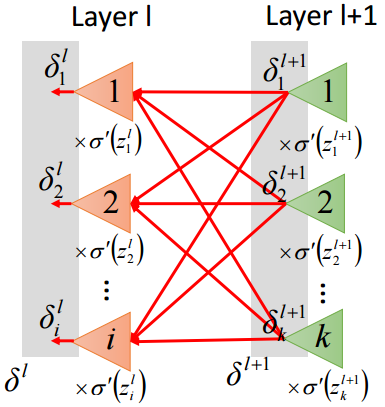
\includegraphics[scale=0.4]{backward}
\end{center}
\[
\delta^l = \sigma^\prime(z^l)\odot[(W^{l+1})^T\delta^{l+1}]
\]
\end{enumerate}

\section{Summary}
Our goal is:
\[
\frac{\partial C_r}{\partial w^l_{ij}} = \frac{\partial C_r}{\partial z^l_i}\frac{\partial z^l_i}{\partial w^l_{ij}}
\]
\[
\frac{\partial z^l_i}{\partial w^l_{ij}}
=
\begin{cases}
x^r_j & \textrm{input layer}\\
a^{l-1}_j & \textrm{hidden layer}
\end{cases}
\]
To compute $\delta^l_i = \frac{\partial C_r}{\partial z^l_i}$, we divide it into two step:
\begin{enumerate}
\item
For output layer $L$:
\[
\delta^L = \nabla C_r(y^r)\odot \sigma^\prime(z^L)
\]
\item
For hidden layers $\delta^{l+1}$ and $\delta^l$:
\[
\delta^l = \sigma^\prime(z^l)\odot [(W^{l+1})^T\delta^{l+1}]
\]
\end{enumerate}
To visualize forward-pass and backward-pass, we have:
\begin{center}
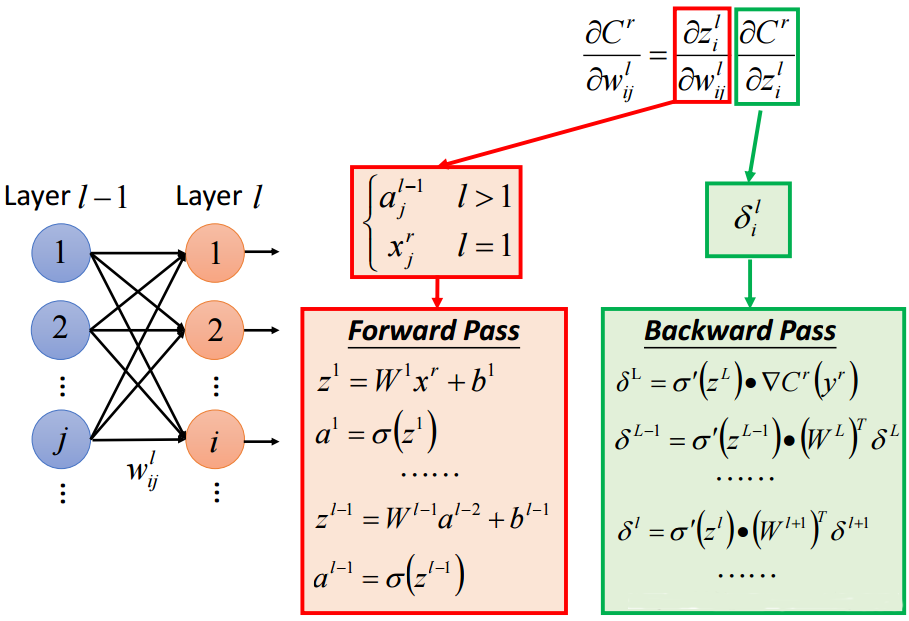
\includegraphics[scale=0.35]{summary}
\end{center}
The black dot in the figure is equivalent to $\odot$ and means element-wise multiplication.

\end{document}